\section{About the Authors}\label{about-the-authors}


\includegraphics[width=1in,height=1.39583in]{./Fig/image1.jpeg}Ralph
Ford obtained his Ph.D. and M.S. degrees in Electrical Engineering from
the University of Arizona in 1994 and 1989 respectively. He obtained his
B.S. in Electrical Engineering from Clarkson University in 1987. He
worked for the IBM Microelectronics Division in East Fishkill, NY from
1989-1991, where he developed machine vision systems to inspect
electronic packaging modules for mainframe computers. Ralph also has
experience working for IBM Data Systems and the Brookhaven National
Laboratory. He joined the faculty at Penn State Erie, The Behrend
College in 1994. Ralph has experience teaching electronics and software
design, as well as teaching the capstone design course sequence in the
electrical, computer, and software engineering programs. His research
interests are in engineering design, image processing, machine vision,
and signal processing. Ralph is currently Director of the School of
Engineering at Penn State Behrend. He also serves as a program evaluator
for ABET. He was awarded a Fulbright Scholarship to study at the Brno
University of Technology in the Czech Republic in 2005.

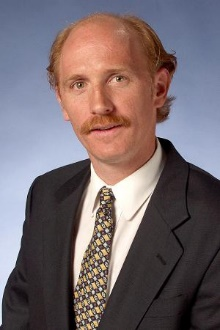
\includegraphics[width=1in,height=1.5in]{./Fig/image2.jpeg}Chris
Coulston obtained his Ph.D. in Computer Science and Engineering from the
Pennsylvania State University in 1999. He obtained his M.S. and B.S in
Computer Engineering from the Pennsylvania State University in 1994 and
1992 respectively. Chris has industry experience working for IBM in
Manassas, VA and Accu-Weather in State College, PA. He joined the
faculty at Penn State Erie, The Behrend College in 1999. He has
experience teaching design-oriented courses in digital systems, embedded
systems, computer architecture, and database management systems. Chris'
research interests are in Steiner tree routing algorithms and artificial
life. He is currently an Associate Professor of Electrical and Computer
at Penn State Behrend and also serves as Chairperson of the program.
